
\chapter{Homework 2}
Show work in all sections. I suggest you utilize MATLAB/Octave for developing functions and plotting (although other languages [Python, R] are allowed). Please include axes labels, units, and titles on all plots. Plot logs vertically (y axis is depth). Please place all results in a single word/pdf file for review. Essay answers should be complete. Please include all functions and scripts in the writeup. You are allowed to discuss the homework assignment with others but every student must turn in their own report and independently develop scripts/codes.

%%%%%%%%%%%%%%%%%%%%%%%%%%%%%%%%%%%%%%%%%%%%%%%%%%%
%        Problem-1: Gas rising from below
%%%%%%%%%%%%%%%%%%%%%%%%%%%%%%%%%%%%%%%%%%%%%%%%%%%

\section{Problem 1: Gas rising from below...}
You are part of a marine seismic crew attempting to image a plume of methane rising through the near-shore sediments. As part of your assignment, you need to perform some forward modeling to better understand the imaging target. This problem will provide an opportunity for you to implement/remember contact theory, fluid substitution, and partial saturation models.


%%%%%%%%% T-1 %%%%%%%%%%
\subsection{The sediment stack}
Your first task is to roughly estimate the velocity structure of the seafloor floor sediment column which is predominantly sandy.

\begin{problem}{(a)}
    Utilize the Hertz-Mindlin model to calculate the expected dry frame moduli (bulk and shear) as a function of depth to 200 m. Assume that the porosity is a constant 36\% and the grains are entirely quartz. Use an appropriate empirical model for calculating coordination number. Estimate stress state assuming a lithostatic gradient of 1 psi/ft and assuming hydrostatic fluid pressure. Please state and justify other assumptions.
\end{problem}
\begin{solution}
    For the appropariate empirical model of coordination number, I used the following formula:
    \begin{align}
        C = C_0 + 9.7 (\phi_0 - \phi)^{0.48}
        \label{equ:Cn}
    \end{align}
    I set $C_0$ equal to $5.3$, $\phi_0$ equal to $0.384$,
    and I assumed that the sediments is spherical grains because they are near-shore sediments and have a very shollow depths. 
    The results figure showing below:
    \begin{figure}[h]
        \centering
        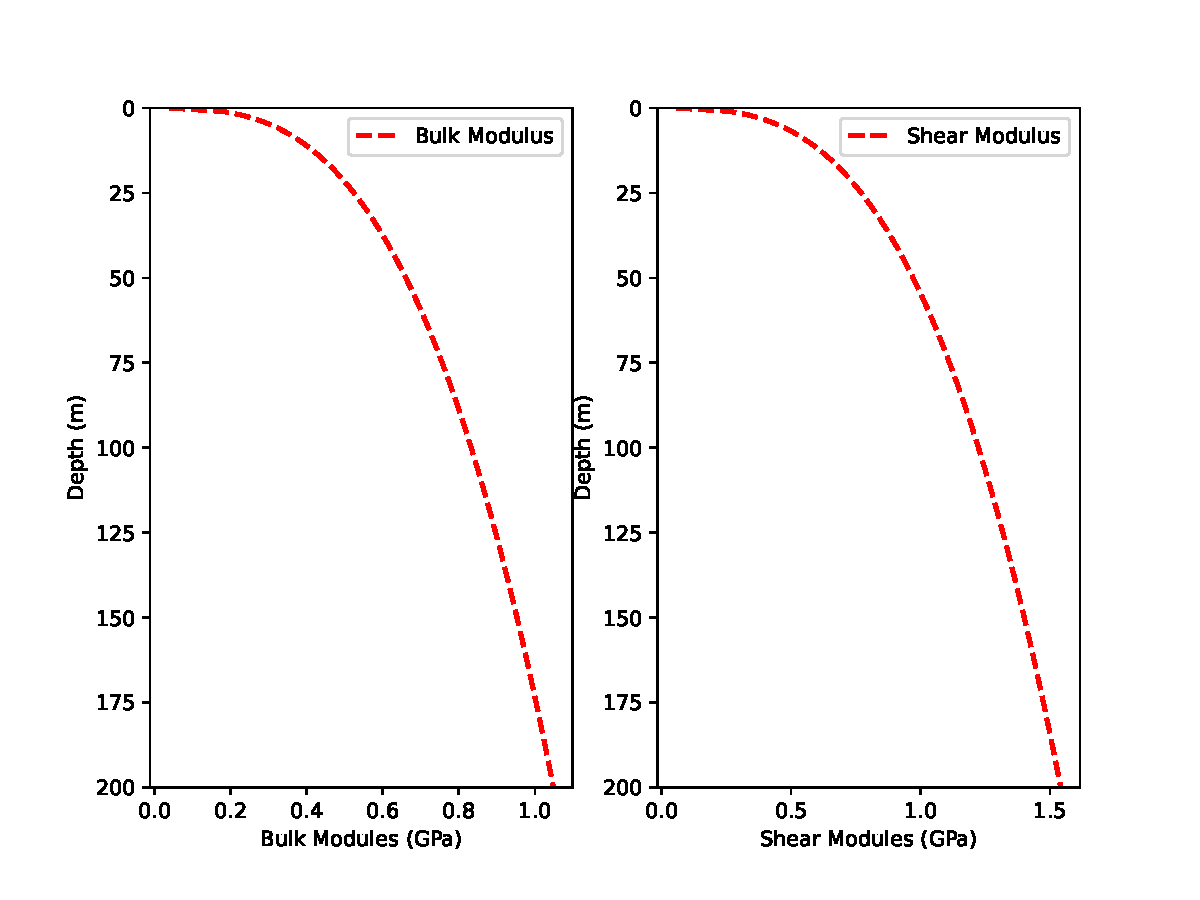
\includegraphics[width=0.8\textwidth]{figures/homework-2/p1-1-a.pdf}
        \caption{Dry frame moduli in depth}
        \label{fig:p1-1-a}
    \end{figure}
\end{solution}


\begin{problem}{(b)}
    Use Gassmann’s model to saturate the profile and assume fresh water (don’t worry about brine). Calculate and plot the saturated $V_p$ , $V_s$ , and $V_p/V_s$ ratio as a function of depth to 200 m.
\end{problem}
\begin{solution}
        \begin{figure}[h]
        \centering
        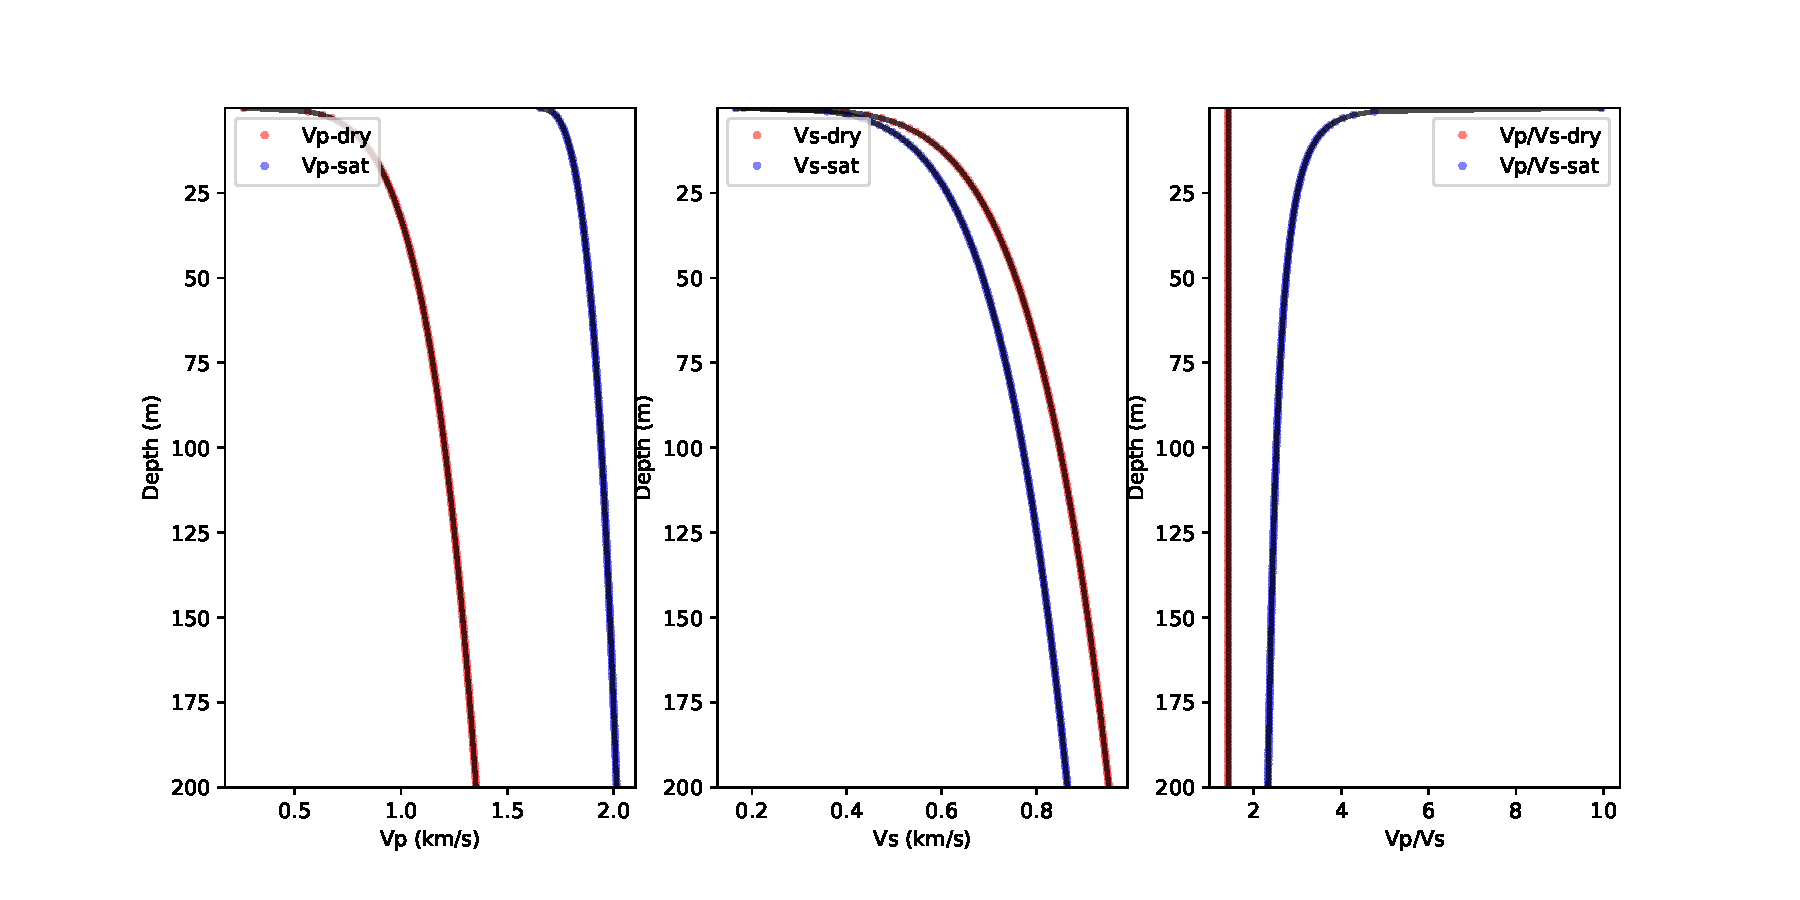
\includegraphics[width=0.8\textwidth]{figures/homework-2/p1-1-b.pdf}
        \caption{Saturated Velocity Model}
        \label{fig:p1-1-b}
    \end{figure}
\end{solution}

%%%%%%%%% T-2 %%%%%%%%%%
\subsection{Partial gas saturation}
While methane is known to be bubbling from the seafloor, the broader methane saturation is not known. Your task is now to estimate the seismic velocity as a function of gas saturation for the methane zone.

\begin{problem}{(a)}
    First, calculate the properties of methane at 100m depth using the methane model described in the RPH, pg. 341-342. Assume \& justify your choice of geothermal gradient.
\end{problem}
\begin{solution}
    According to some papers, I assumed that the temperature gradient is $0.02^{\circ}C/m$ in shallow depth,
    and also assuming a lithostatic gradient of $1 psi/ft$.
\begin{pythoncode}
## Compute
G = 0.56; depth = 100  # in m
P = P0 + 1/0.3048*6.8947572932e-6*depth # in GPa 
d = 100; tg = 0.02
KG, pG = gas_bulk(G,P,d,tg)
print('KG = ', KG)
## Output
KG =  0.002986930151536351
\end{pythoncode}
\end{solution}



\begin{problem}{(b)}
    Next, use the two effective fluid models discussed in class (patchy and well-mixed) to calculate the properties of the mixed fluids. Plot the effective fluid modulus as a function of gas/water fraction. Assume fresh water with a density of 1 g/cc and a velocity of 1500 m/s.
\end{problem}
\begin{solution}
    I used two effective fluid models, patchy and well-mixed respectively.
    \begin{figure}[H]
        \centering
        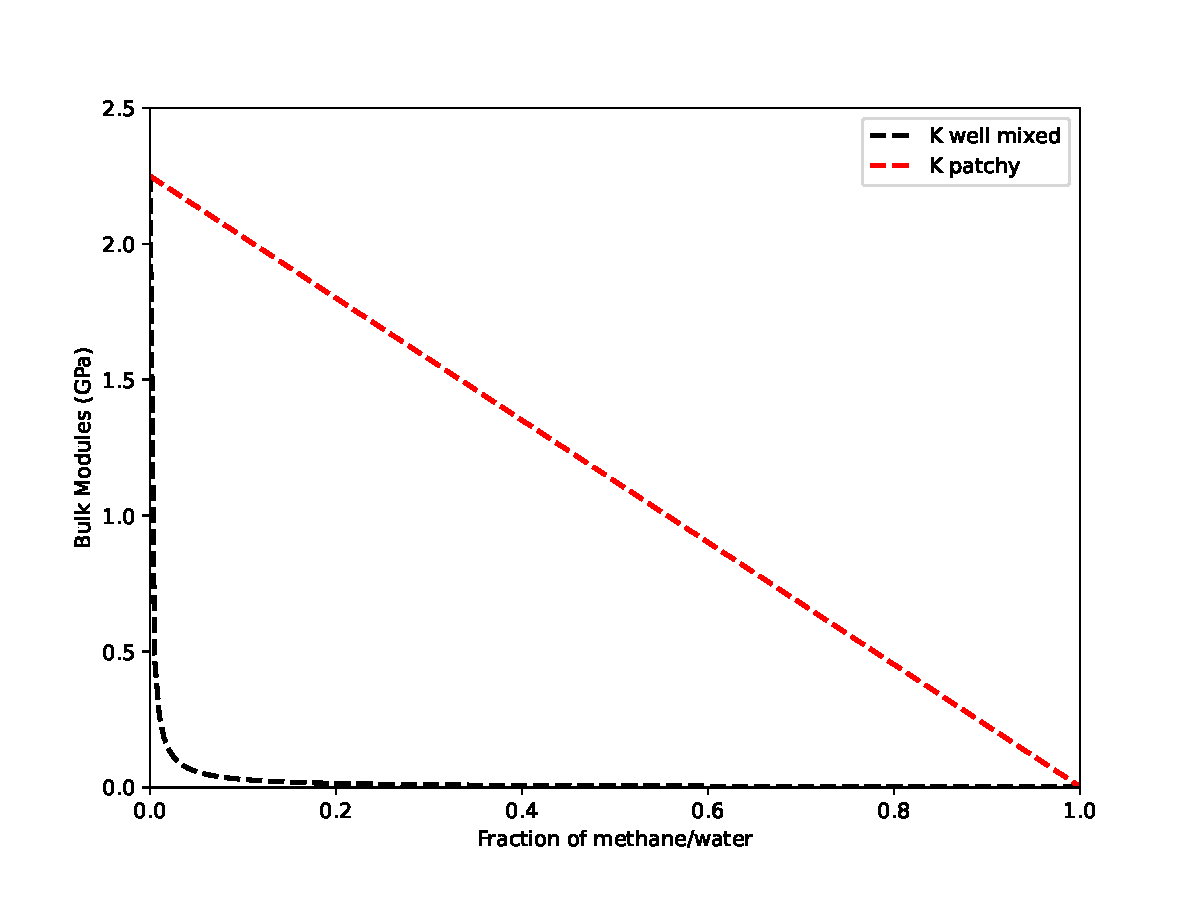
\includegraphics[width=0.6\textwidth]{figures/homework-2/p1-2-b.pdf}
        \caption{Effective fluid models, patchy and well-mixed respectively}
        \label{fig:p1-2-b}
    \end{figure}
\end{solution}



\begin{problem}{(c)}
    Using these effective fluid models, calculate the Vp, Vs, and Vp/Vs profiles. Assume a 10 m gas sand starting at a depth of 100 m from the seafloor. Calculate depth profiles at several assumed saturations (0-100%). Also calculate curves for Vp, Vs, and Vp/Vs as a function of methane saturation.
\end{problem}
\begin{solution}
    \begin{figure}[H]
        \centering
        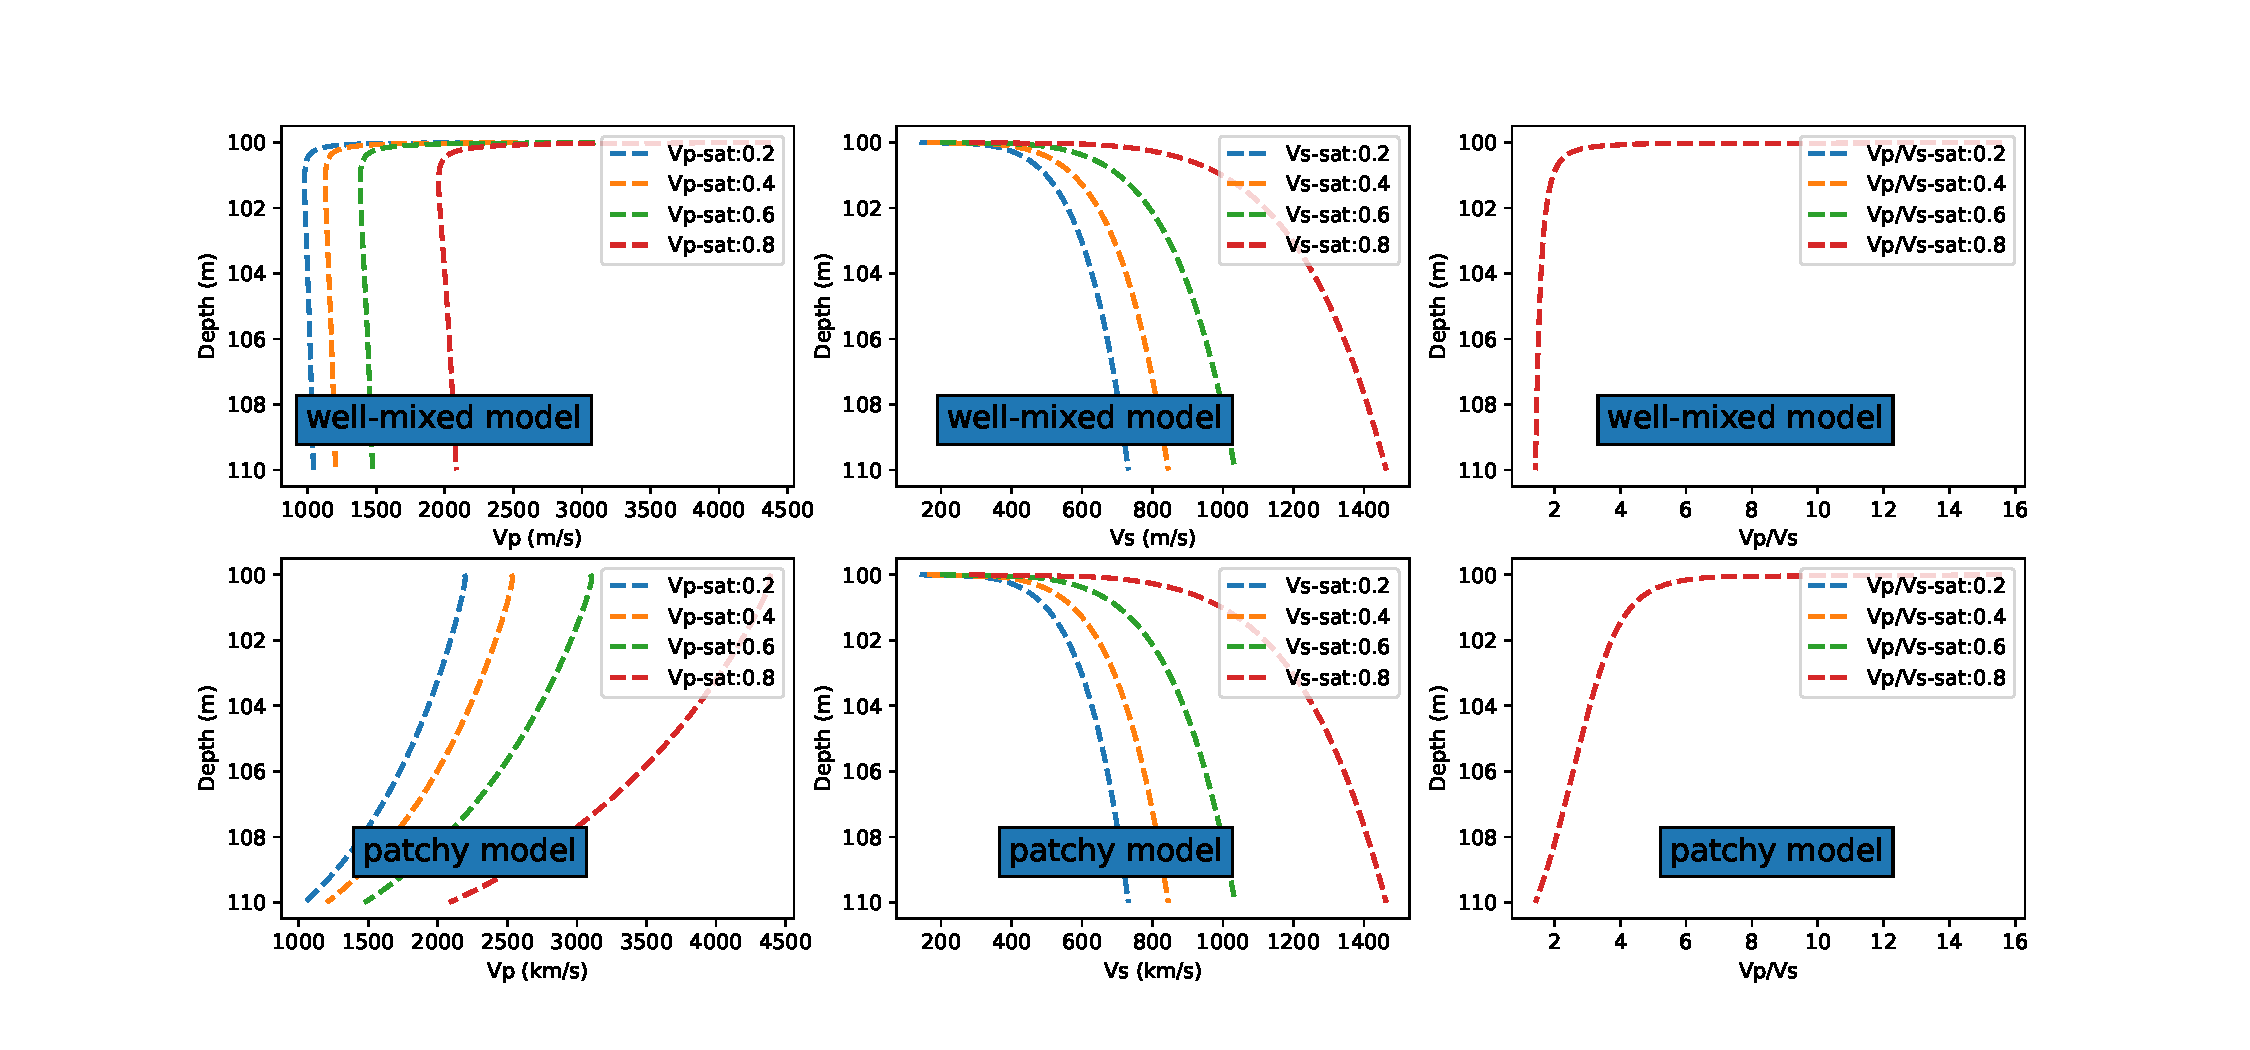
\includegraphics[width=1.0\textwidth]{figures/homework-2/p1-2-c1.pdf}
        \caption{Depth profiles at several assumed saturations}
        \label{fig:p1-2-c1}
    \end{figure}
    \begin{figure}[H]
        \centering
        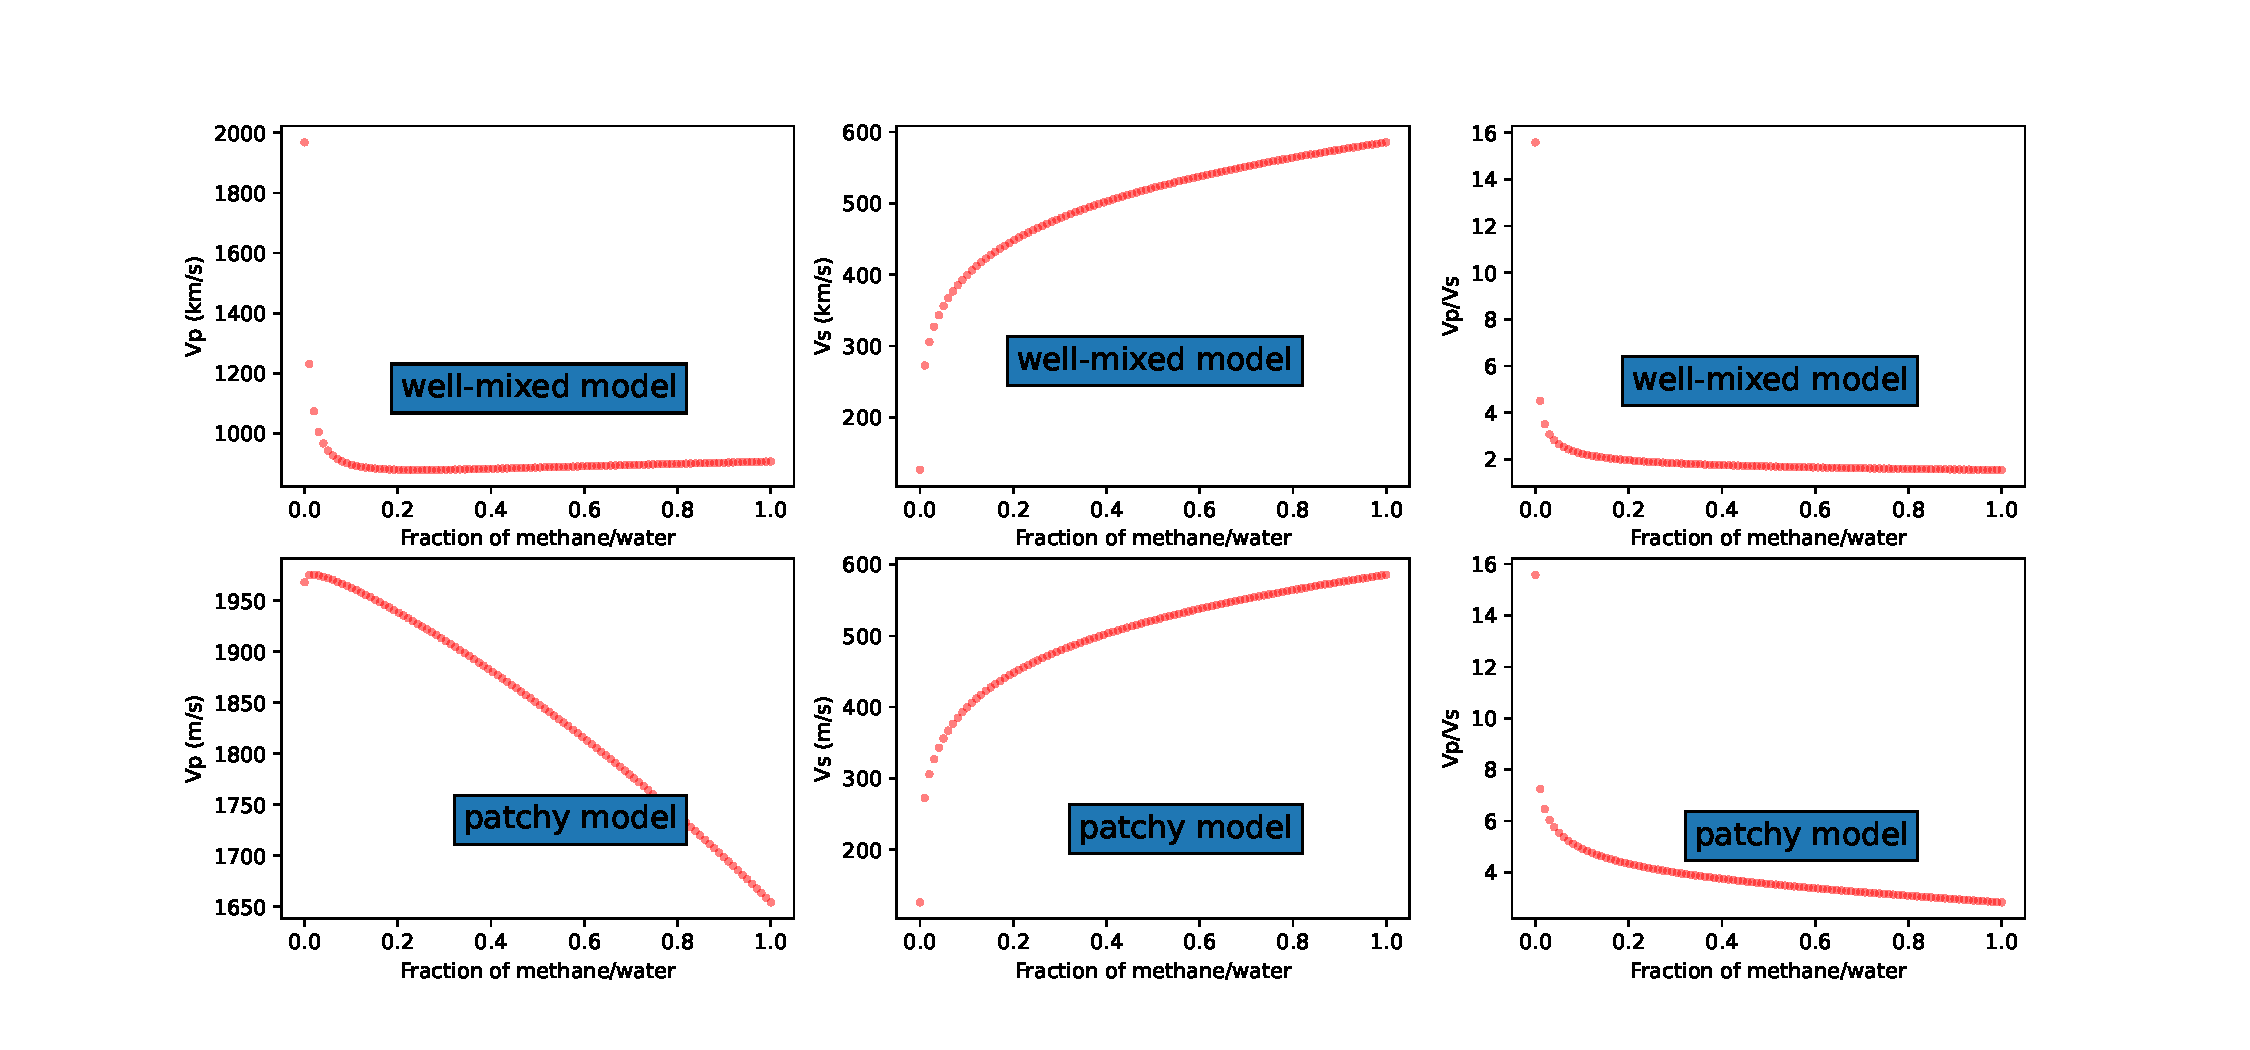
\includegraphics[width=1.0\textwidth]{figures/homework-2/p1-2-c2.pdf}
        \caption{Vp, Vs, and Vp/Vs as a function of methane saturation}
        \label{fig:p1-2-c2}
    \end{figure}
\end{solution}


%%%%%%%%% T-3 %%%%%%%%%%
\subsection{Reflections from the gassy zone}
Now that you have models for the velocity variations in the gassy layer, you need to estimate the likely signature

\begin{problem}{(a)}
    First, calculate the impedance values for the partially saturated unit as a function of methane saturation.
\end{problem}

\begin{solution}
    \begin{figure}[H]
        \centering
        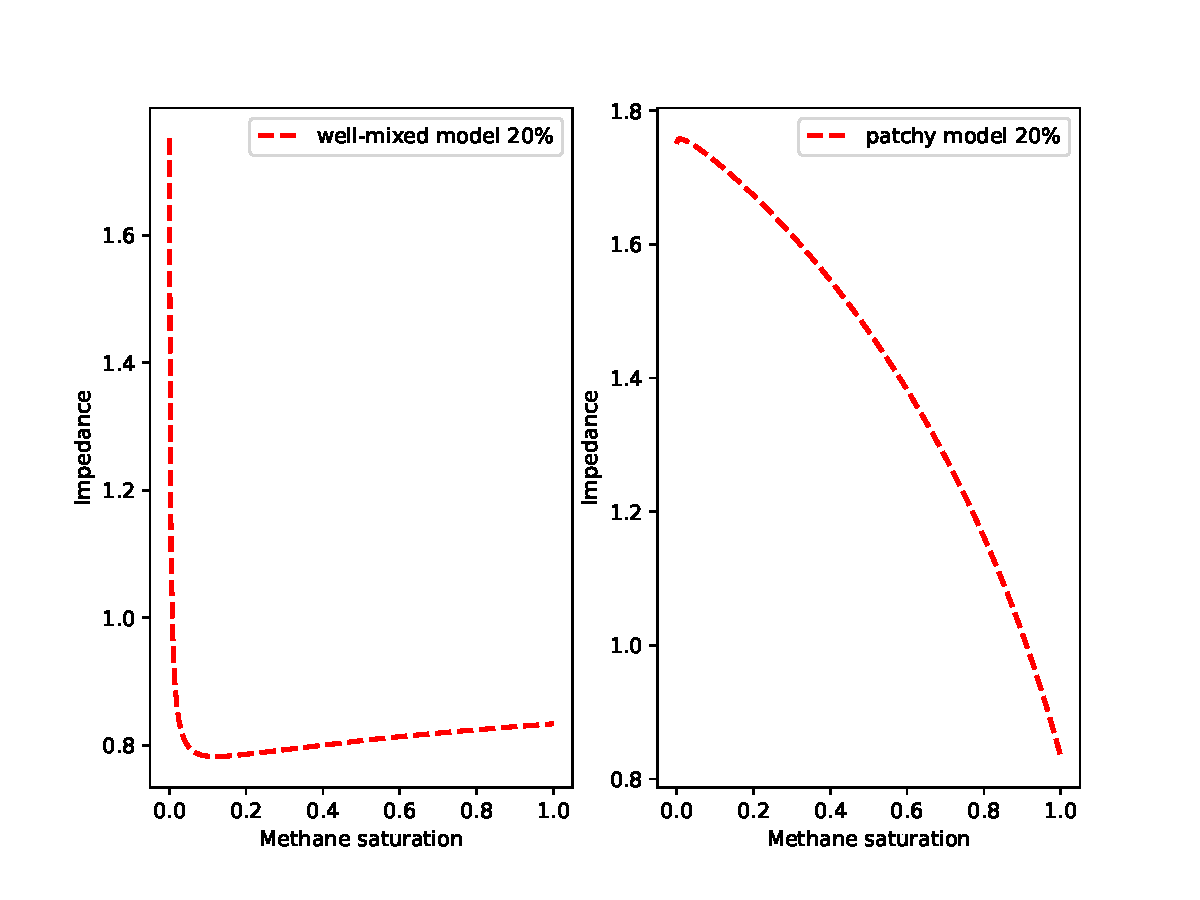
\includegraphics[width=0.8\textwidth]{figures/homework-2/p1-3-a.pdf}
        \caption{Impedance}
        \label{fig:p1-3-a}
    \end{figure}
\end{solution}

\begin{problem}{(b)}
    Next, calculate the normal incidence angle P and S wave reflectivity as a function of gas saturation. Make these calculations for the top of the gas interval.
\end{problem}

\begin{solution}
    \begin{figure}[H]
        \centering
        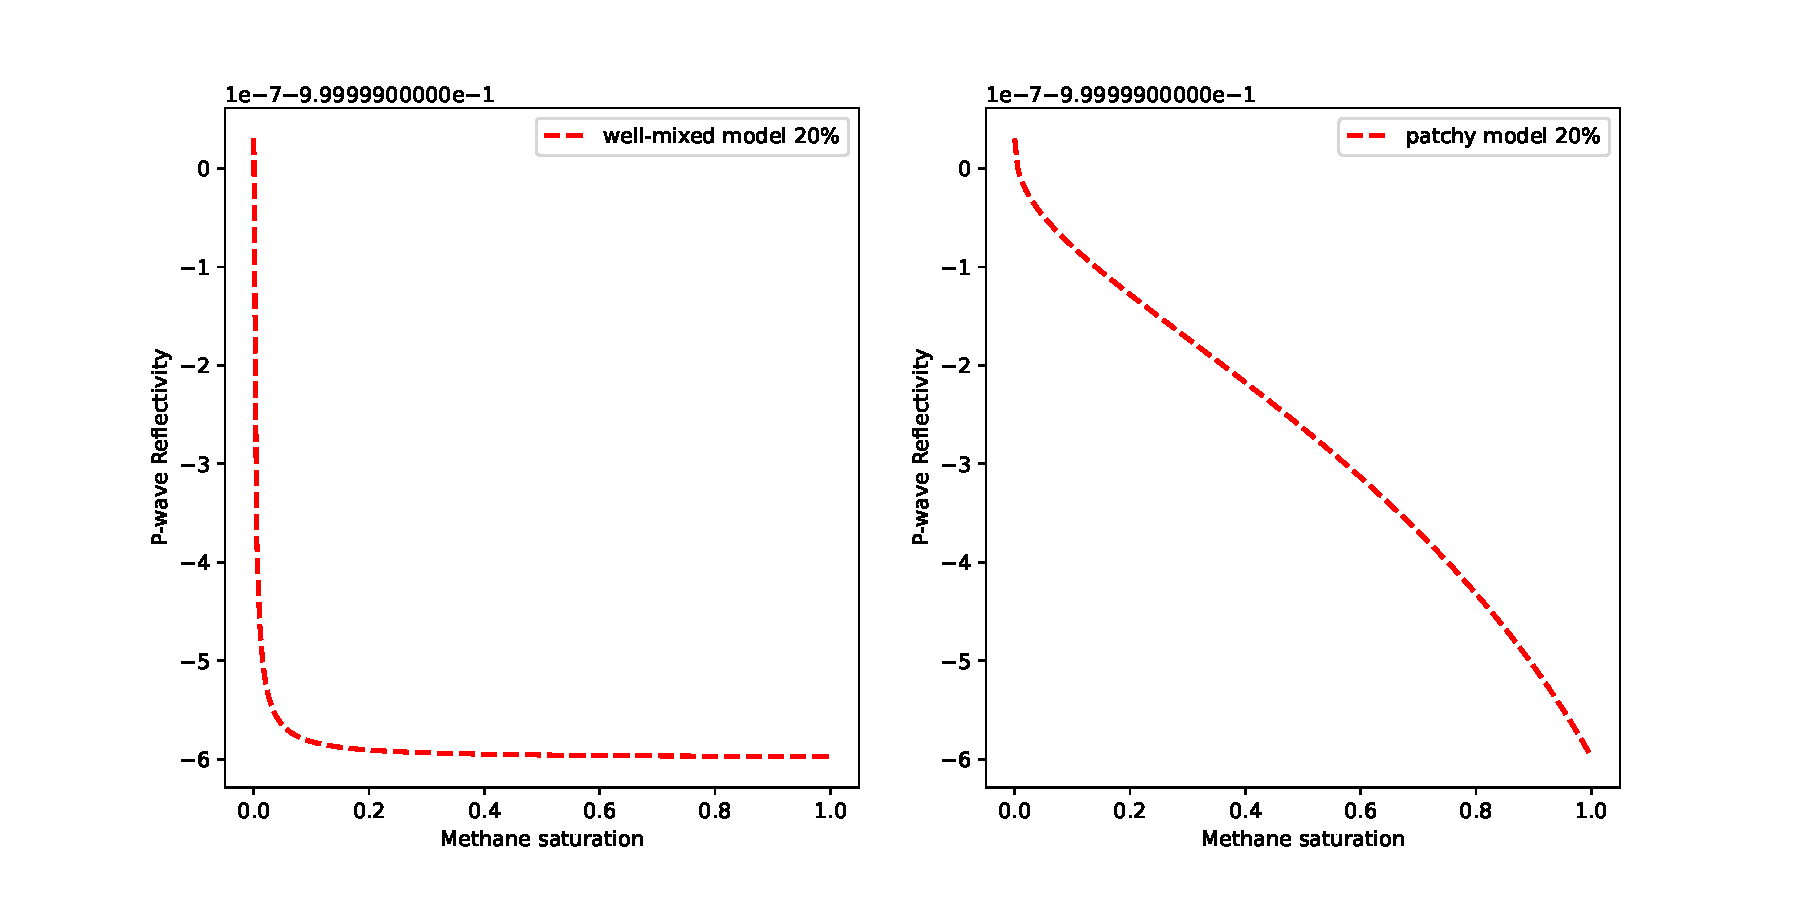
\includegraphics[width=1.0\textwidth]{figures/homework-2/p1-3-b1.pdf}
        \caption{P wave reflectivity}
        \label{fig:p1-3-b1}
    \end{figure}
    \begin{figure}[H]
        \centering
        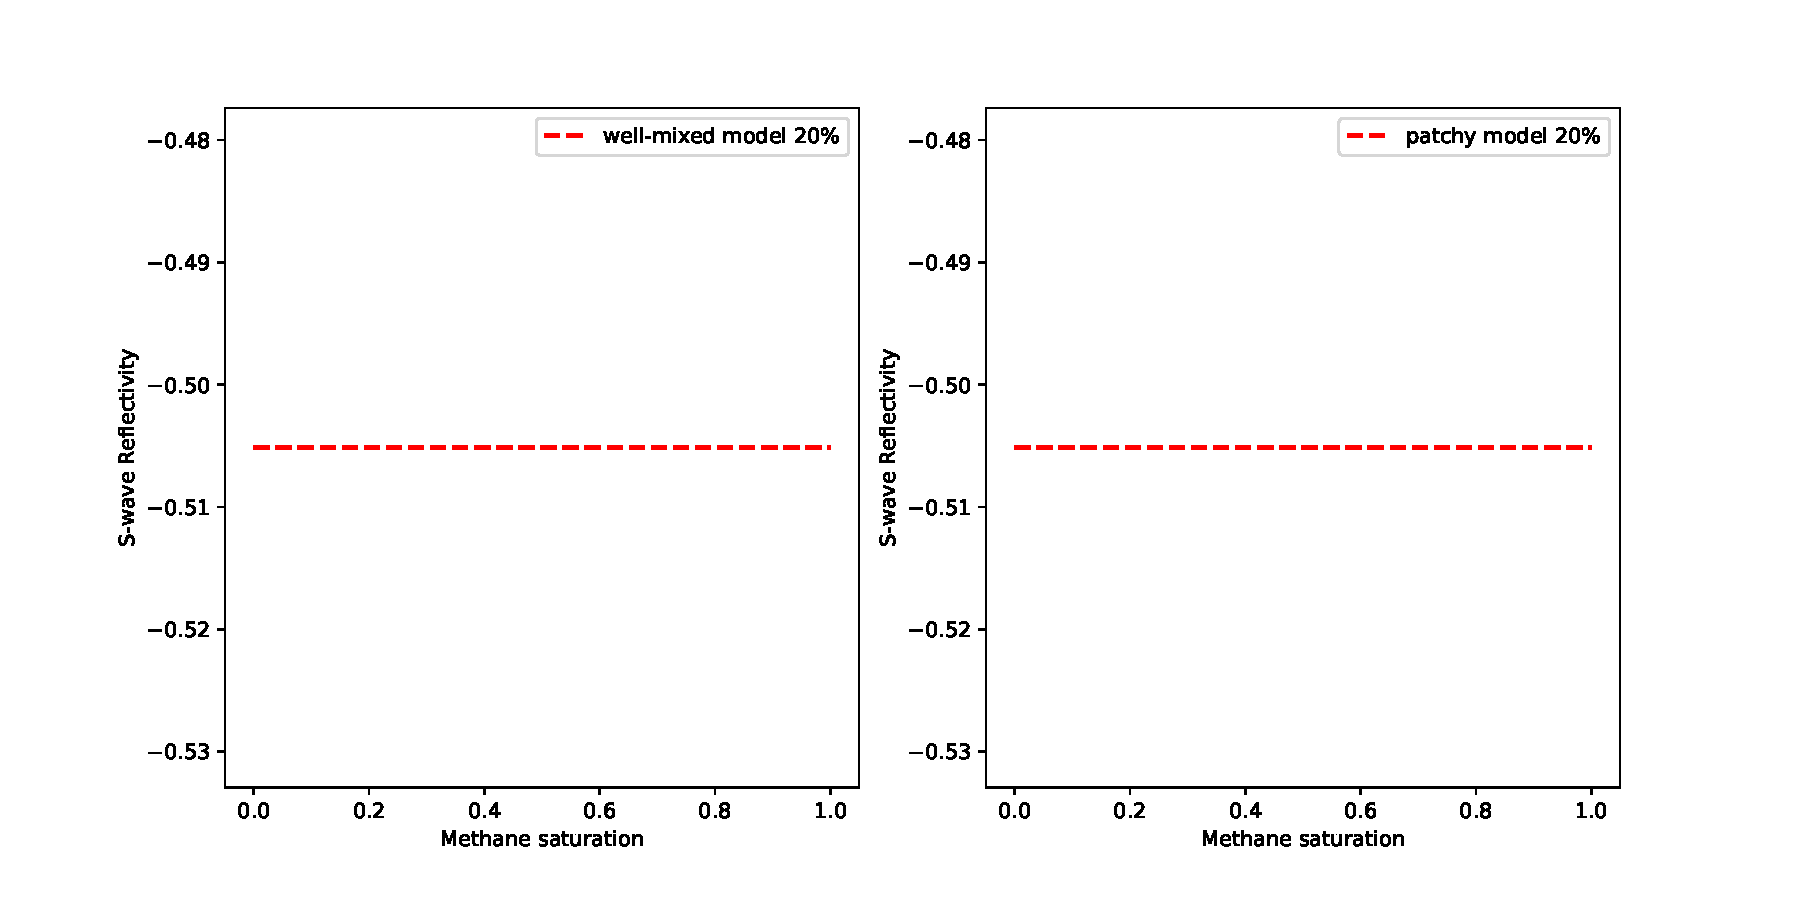
\includegraphics[width=1.0\textwidth]{figures/homework-2/p1-3-b2.pdf}
        \caption{S wave reflectivity}
        \label{fig:p1-3-b2}
    \end{figure}
\end{solution}


\begin{problem}{(c)}
    Assume that a normal reflectivity of 0.1 is required to image the reflector. What gas saturation would be detectable in this scenario?
\end{problem}

\begin{solution}
    Something is wrong in this question, and I need to figure out it later.
\end{solution}


%%%%%%%%%%%%%%%%%%%%%%%%%%%%%%%%%%%%%%%%%%%%%%%%%%%
%    Problem-2: Stiff Inclusions and Sandstones
%%%%%%%%%%%%%%%%%%%%%%%%%%%%%%%%%%%%%%%%%%%%%%%%%%%

\section{Problem 2: Stiff Inclusions and Sandstones}
In this problem, you will explore the properties of inclusion effective medium models, in particular the self-consistent model of Budiansky (RPH page 185-187, 2 nd edition). Use the randomly oriented penny-shaped crack model for these exercises

\begin{problem}{(a)}
    Code up the Budiansky SC model for experimentation. You may use the explicit linear assumption between crack density and cracked solid Poisson’s ratio.
\end{problem}
\begin{solution}
    Please check the code.

\begin{pythoncode}
import np as np

def budiansly(crack_radius, K, mu, a, ncracks_per_volume):
"""
Calculate the Budiansky Self-Consistency model.

Parameters
----------
    crack_radius : float
        Crack's radius in cm.
    K : float
        Bulk modulus.
    mu : float
        Shear modulus.
    a : float 
        Aspect ratio.
    ncracks_per_volume : float or array
        The number of cracks per unit volume
        
Returns
-------
    k_dry : float or array
        Dry bulk modulus.
    mu_dry : float or array
        Dry shear modulus.
    porosity: float or array
        Porosity.
    
"""
e = ncracks_per_volume*crack_radius**3
v = ((3*K)-(2*mu))/(2*(3*K+mu))
v_sc = v*(1-((16/9)*e))
Kdry = K*(1-(((16/9)*((1-v_sc**2)/(1-(2*v_sc))))*e))
mudry = mu*(1-(((32/45)*(((1-v_sc)*(5-v_sc))/(2-v_sc)))*e))
porosity = 4*pi*a*e/3

return Kdry, mudry, porosity
\end{pythoncode}
\end{solution}


\begin{problem}{(b)}
    Construct a plot of the dry bulk modulus, Kdry, and shear modulus (Gdry) for a quartz sandstone assuming a crack length, c, of 1 mm, against the number of cracks per unit volume (N/Vbulk) from 0 to 1000 (assume a cell size of 1 cm). What happens to the moduli if you change the crack length, c, to 2 mm?
\end{problem}
\begin{solution}
    I find that both bulk and shear modulus will be decreased when increasing the crack length.
    \begin{figure}[H]
        \centering
        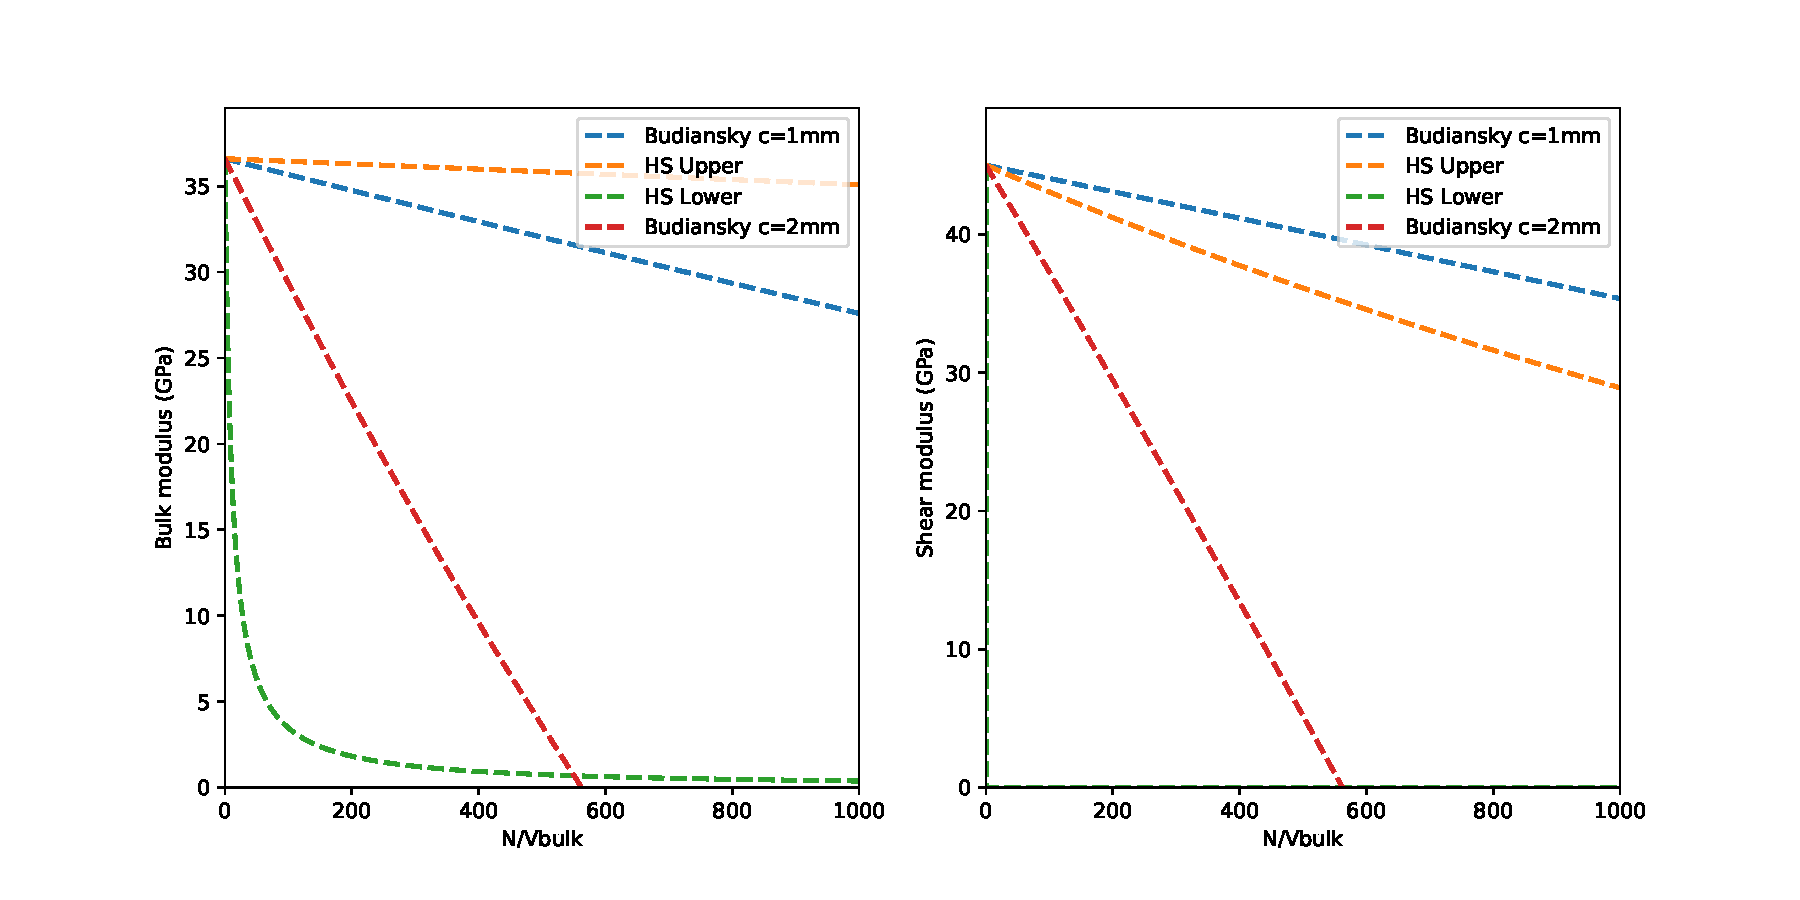
\includegraphics[width=1\textwidth]{figures/homework-2/p2-b.pdf}
        \caption{Impedance}
        \label{fig:p2-b}
    \end{figure}
\end{solution}



\begin{problem}{(c)}
    Plot the dry bulk modulus, Kdry, against porosity (from 0 to 0.4) using the porosity definition of crack density, assuming an aspect ratio of 0.05. Also plot the HashinShtrikman bounds for the same phase combinations. How does the SC model compare to the bounds? Using both what you have learned in class and this example, over what domain do you think the model is useful? Why do you think the approximation breaks down?
\end{problem}
\begin{solution}
    Compared with Hashin-Shtrikman model, the SC model is between the bounds.
    And when less than the critical porosity, the SC model is meaningful.
    The reason why SC model is broken down is that not consider some other suspensions.
    \begin{figure}[H]
        \centering
        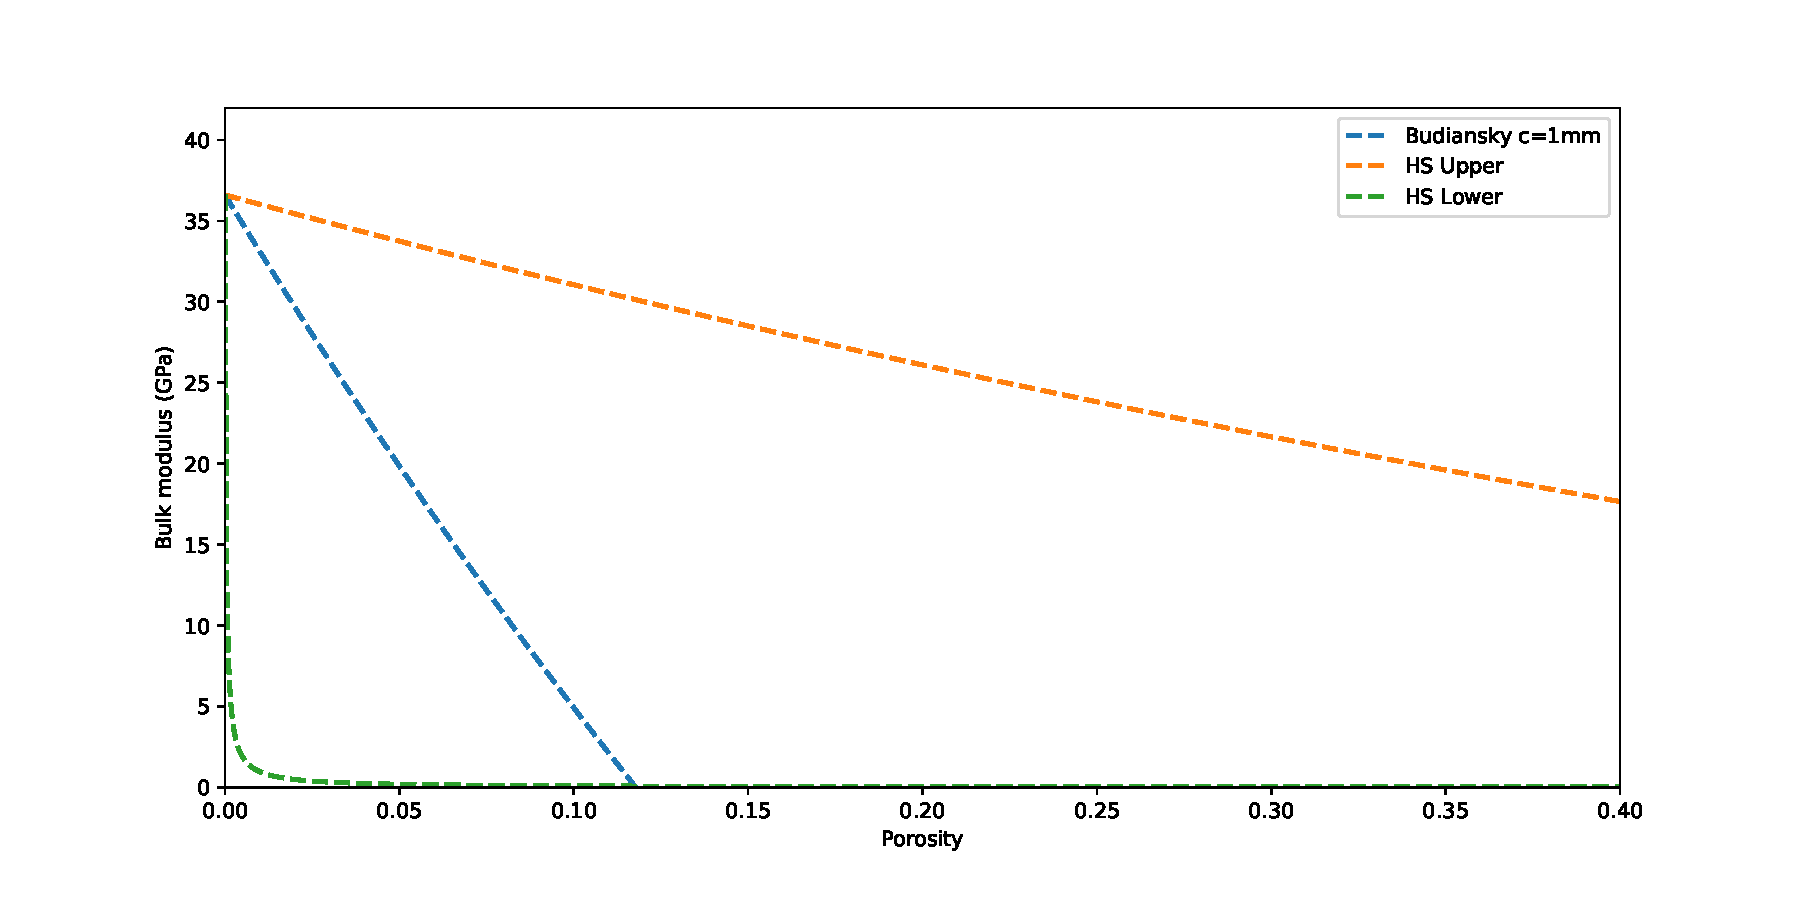
\includegraphics[width=1\textwidth]{figures/homework-2/p2-c.pdf}
        \caption{Impedance}
        \label{fig:p2-c}
    \end{figure}
\end{solution}



\begin{problem}{(d)}
    Calculate the Vp values for the dry example with 2mm cracks in terms of porosity. If you have a rock sample (again, you can assume a pure quartz sandstone) with a Vp of 4100 m/sec, a Vs of 2400 m/sec, a porosity of 0.2, how many cracks do you think it has per unit volume.
\end{problem}
\begin{solution}
    Vp values is showing below
    \begin{figure}[H]
        \centering
        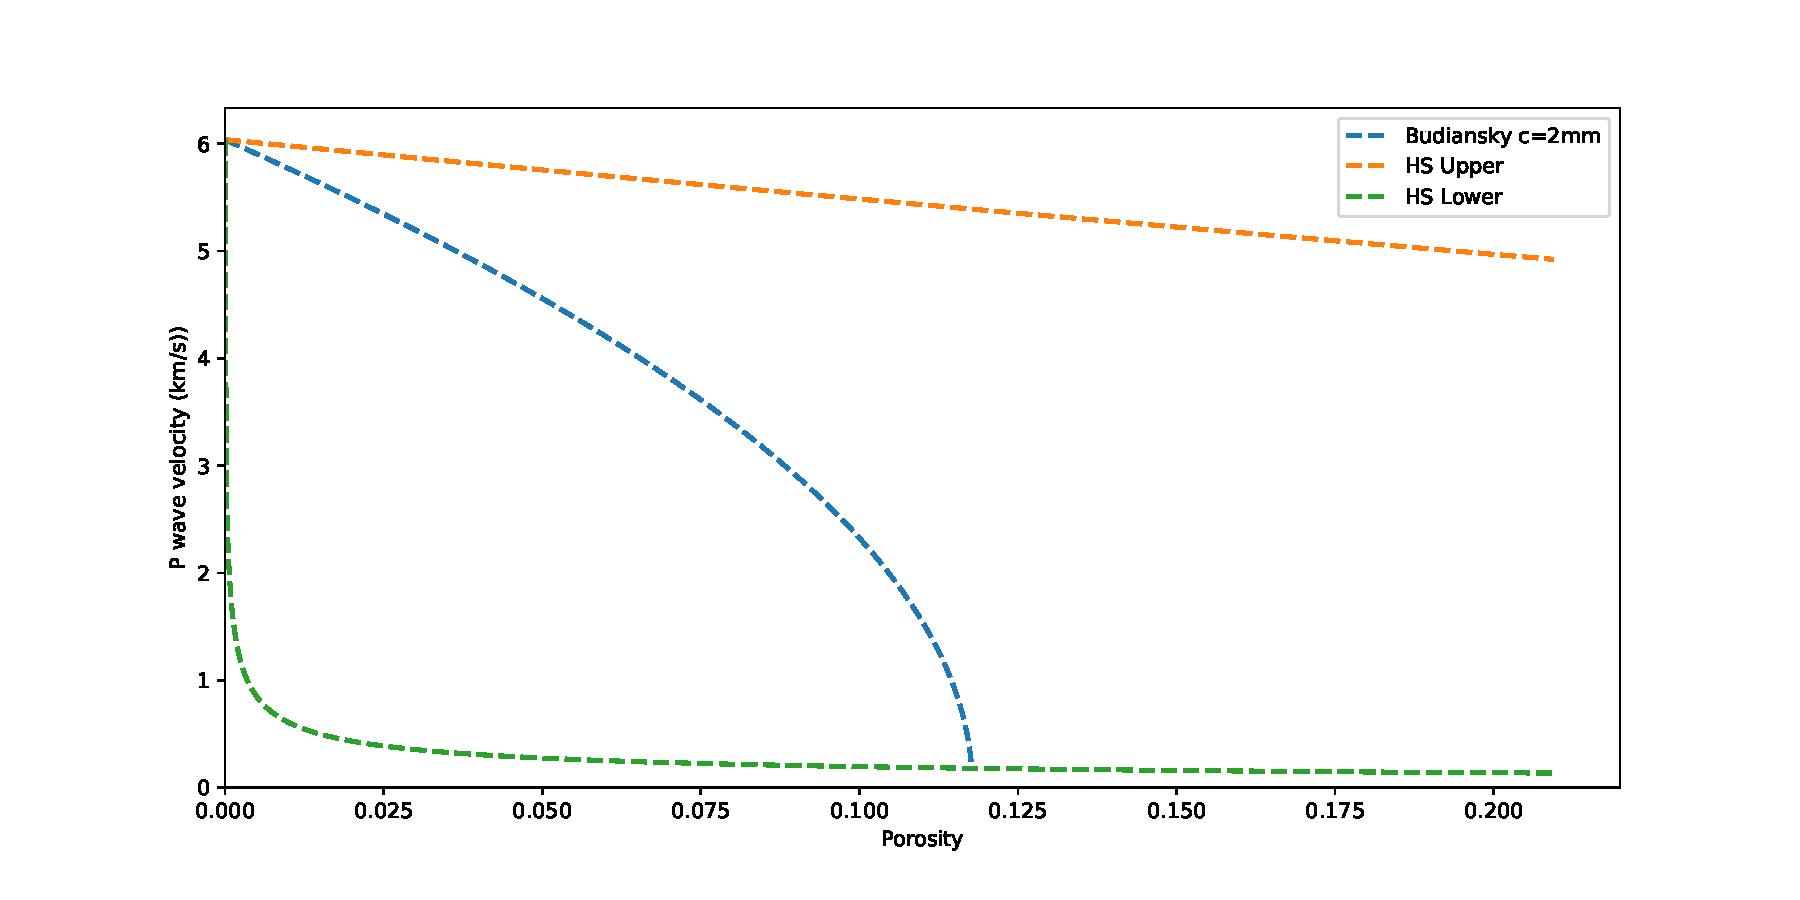
\includegraphics[width=1\textwidth]{figures/homework-2/p2-d.pdf}
        \caption{Impedance}
        \label{fig:p2-d}
    \end{figure}

    According to the formula:
    \begin{align}
        \varepsilon  & = \frac{3\phi }{4\pi \alpha }  \\
        \varepsilon  & = \frac{N }{V_{bulk} } (\frac{c}{2})^3
        \label{equ:varepsilon}
    \end{align}
    where $\phi = 0.2$, $c=0.2$  $\alpha=0.05$, we can get the number of cracks per unit volume 
    is 955.414, and so the is approximate number is 955.
\end{solution}




\begin{problem}{(e)}
    Load up the data we used in HW 1, Use the Data.mat file from the Canvas site. Select the water-saturated Vp, Vs, density, porosity, and clay content data for 30 and 40 MPa. Discard the rest of the data. After you have the data for 30 and 40 MPa, select only the clean sandstones (Clay < 15\%). Extract the porosity and dryVp40 columns for comparisons.
\end{problem}
\begin{solution}
    \begin{figure}[H]
        \centering
        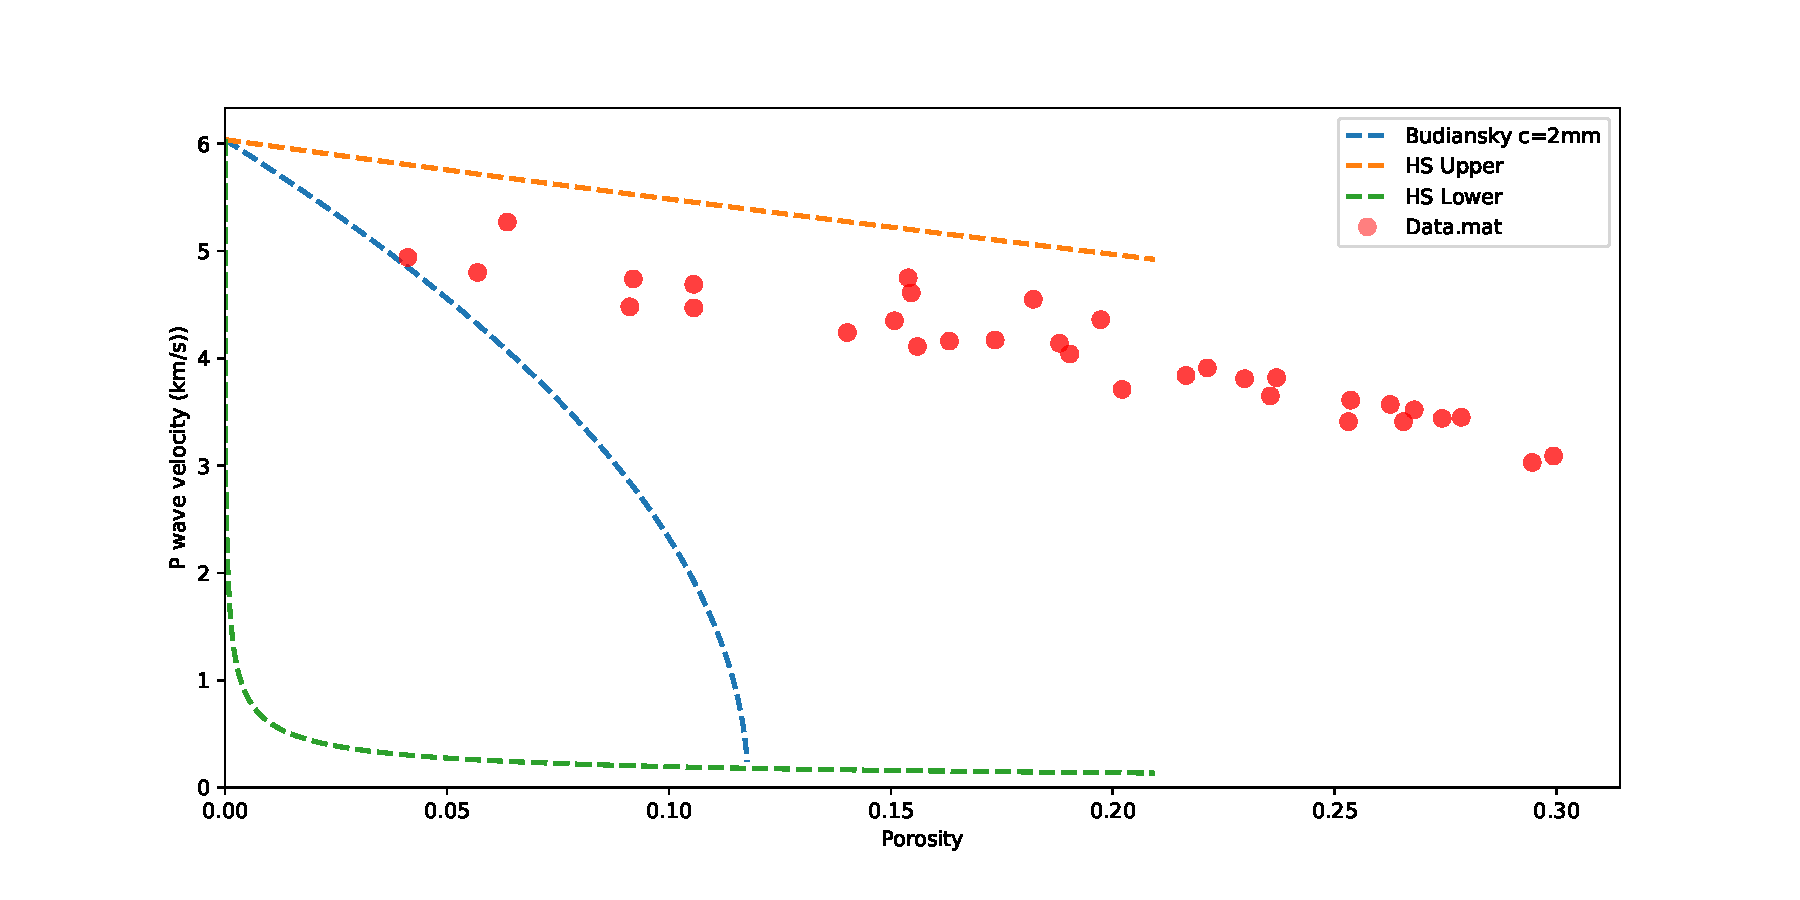
\includegraphics[width=1\textwidth]{figures/homework-2/p2-e.pdf}
        \caption{Impedance}
        \label{fig:p2-e}
    \end{figure}
\end{solution}

\begin{problem}{(f)}
    Using the porosity formulation for crack density, what pore aspect ratio best fits the Vp/porosity trends in the clean sandstone data? Plot a comparison between the model and the dataset. What discrepancies exist between the model and the dataset? Why might they be present?
\end{problem}
\begin{solution}
    I find when aspect ratio is 0,15, the data will be fitted well.
    Dataset is scattered on both sides of the SC model, I think it because we set the assumptions for SC model,
    such as idealized ellipsoidal inclusion shapes and isotropic, linear and elastic media.
    \begin{figure}[H]
        \centering
        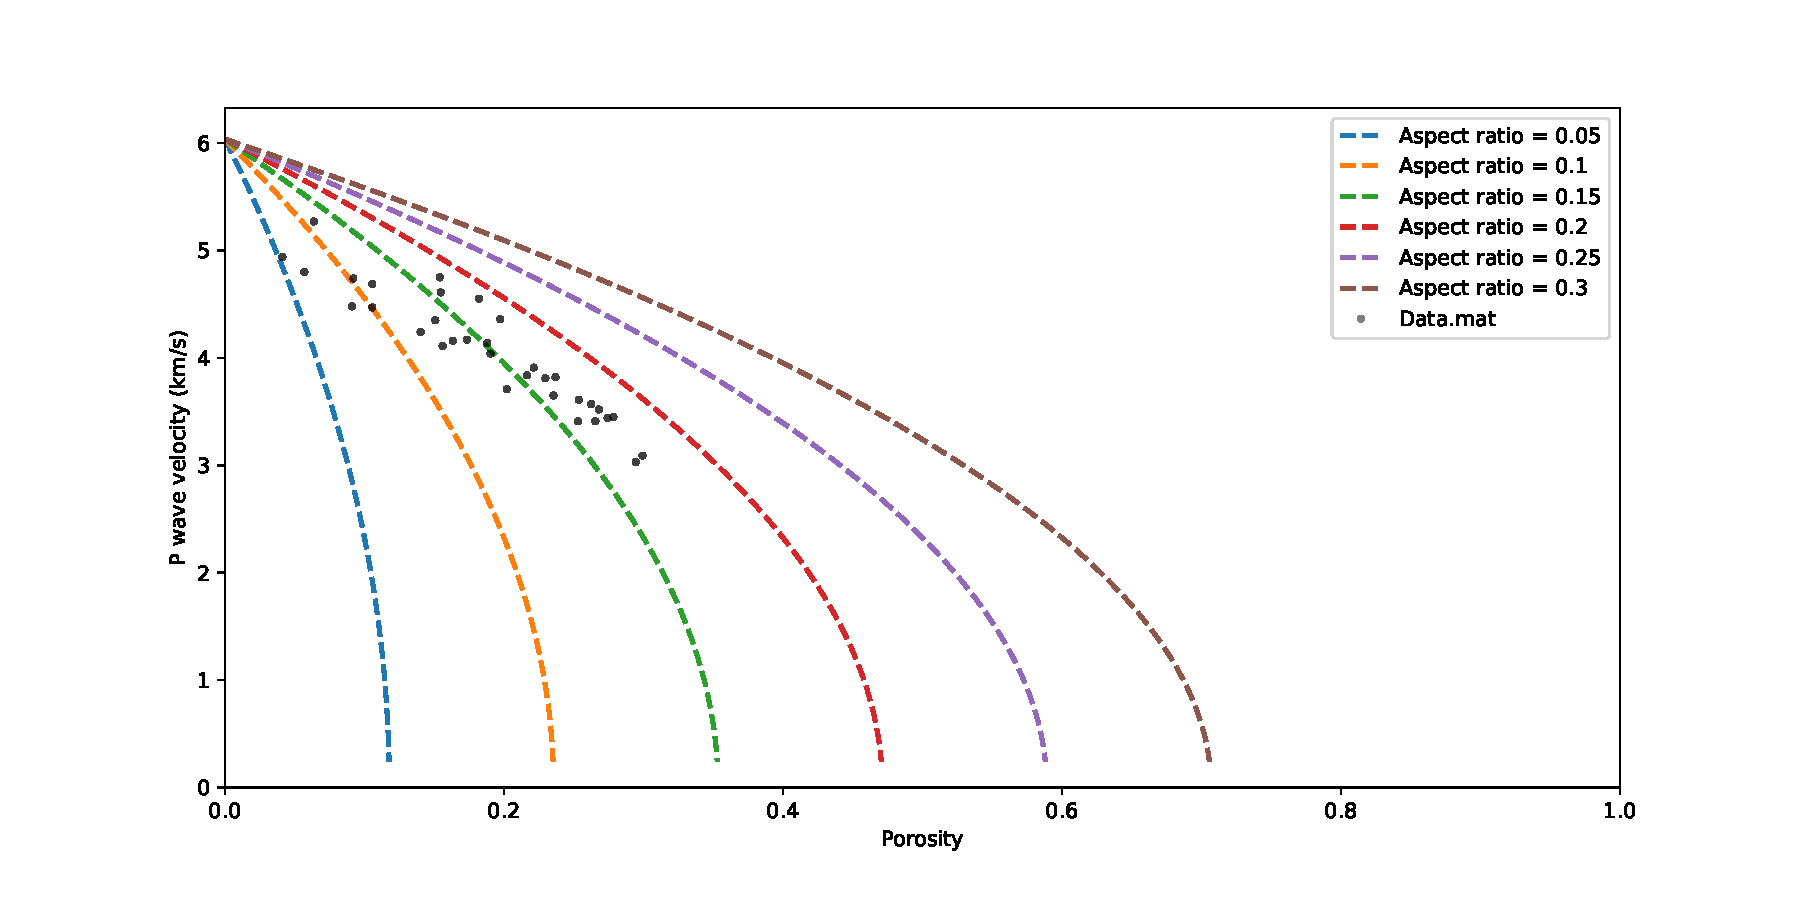
\includegraphics[width=1\textwidth]{figures/homework-2/p2-f.pdf}
        \caption{Impedance}
        \label{fig:p2-f}
    \end{figure}
\end{solution}



%%%%%%%%%%%%%%%%%%%%%%%%%%%%%%%%%%%%%%%%%%%%%%%%%%%
% Problem-3: Understanding the Anisotropy of Organic-Rich Shales
%%%%%%%%%%%%%%%%%%%%%%%%%%%%%%%%%%%%%%%%%%%%%%%%%%%
\section{Problem 3: Understanding the Anisotropy of Organic-Rich Shales}

Shales and other tight grained sediments are important both economically (for unconventional energy production) and as sealing formations for geologic CO 2 storage. These formations also tend to be anisotropic (seismic properties depend on propagation angle) due to the presence of thin compliant layers (organic matter, clay etc). The degree of anisotropy is a useful indicator and must also be incorporated to image below these units without distortion. In this exercise you will explore a set of lab measurements on organic-rich shales from the Bakken formation obtained from the Williston Basin (North Dakota) and experiment with Backus averaging.

Note: In the attached data files, 0 degrees are measurements orthogonal to layering while 90 degrees are parallel to layering. Table 1 includes basic chemical information including kerogen content while Table 2 includes ultrasonic measurements of Vp, Vsh, and Vsv as a function of angle. The ultrasonic measurements were conducted at 70 MPa confining pressure.




\begin{problem}{(a)}
    Develop a short code for computing the Backus average of a 2-phase laminar system. For this exercise, assume that both layers are isotropic. You may use the formulation of Levin (1979) from the RPH (pg 276, ver. 3) which describes the Backus average in terms of Vp, Vs, and rho and yields the horizontal and vertical P and Sh wave velocities. Alternatively, you can use the stiffness (Cij ) formulation and then calculate the appropriate phase velocities at 0 and 90 degrees. Test your code against the worked example in RPH.
\end{problem}

\begin{solution}
    Please check the code.
\begin{pythoncode}
## Function
import numpy as np
def backus_average(vp1, vs1, rho1, h1, vp2, vs2, rho2, h2):
    f1 = h1/(h1+h2)
    f2 = h2/(h1+h2)
    A = f1*4*rho1*vs1**2*(1 - vs1**2/vp1**2) \
        + (f2*4*rho2*vs2**2) * (1-(vs2**2/vp2**2)) \
        + ((f1*(1-(2*vs1**2/vp1**2)) + f2*(1-(2*vs2**2/vp2**2)))**2 * (1/((f1/(rho1*vp1**2)) + (f2/(rho2*vp2**2)))))
    C = 1 / ((f1/(rho1*vp1**2)) + (f2/(rho2*vp2**2)))
    D = 1 / ((f1/(rho1*vs1**2)) + (f2/(rho2*vs2**2)))
    F = (f1*(1-(2*vs1**2/vp1**2)) + f2*(1-(2*vs2**2/vp2**2))) * (1/((f1/(rho1*vp1**2))+(f2/(rho2*vp2**2))))
    M = f1*rho1*vs1**2 + f2*rho2*vs2**2
    B = A - 2*M
    
    return A, B, C, D, F, M

## Test
vp1 = 5200; vs1 = 2700; rho1 = 2450; h1 = 0.75
vp2 = 2900; vs2 = 1400; rho2 = 2340; h2 = 0.5
A, B, C, D, F, M = backus_average(vp1, vs1, rho1, h1, vp2, vs2, rho2, h2)
print('A: '+str(round(A*1e-9,2))+'GPa') 
print('B: '+str(round(B*1e-9,2))+'GPa')
print('C: '+str(round(C*1e-9,2))+'GPa')
print('D: '+str(round(D*1e-9,2))+'GPa')
print('F: '+str(round(F*1e-9,2))+'GPa')
print('M: '+str(round(M*1e-9,2))+'GPa')

## Output
A: 45.11GPa
B: 20.01GPa
C: 34.03GPa
D: 8.28GPa
F: 16.68GPa
M: 12.55GPa
\end{pythoncode}
\end{solution}


\begin{problem}{(b)}
    Load the Bakken shale data from Vernik and Nur (tables 1 and 2) and plot the horizontal and vertical P and SH wave velocity as a function of kerogen content, a soft organic phase often present in hydrocarbon source rock. Documentations as to the units and measurements are in the header for each file.
\end{problem}
\begin{solution}
    \begin{figure}[H]
        \centering
        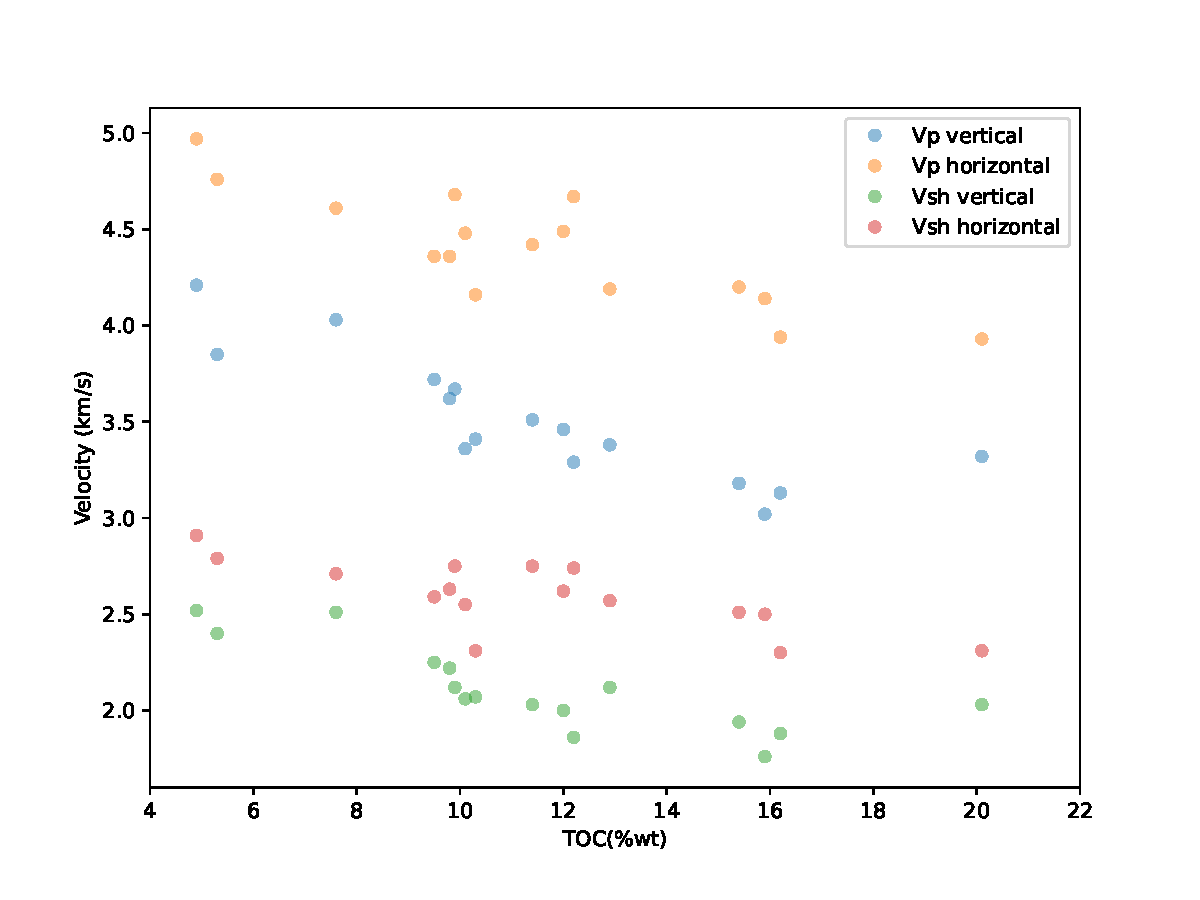
\includegraphics[width=0.8\textwidth]{figures/homework-2/p3-b.pdf}
        \caption{Bakken shale data}
        \label{fig:p3-b}
    \end{figure}
\end{solution}



\begin{problem}{(c)}
    Assume that the kerogen and non-kerogen phases in the shale are isotropic with each having Vp, Vs, and density of (Kerogen: 2700 m/s, 1500 m/s, 1400 kg/m3) and (non-kerogen: 4750 m/s, 3000 m/s, 2700 kg/m3) respectively. Using Backus averaging, compute the predicted horizontal and vertical P and SH wave velocities as a function of kerogen content and compare to the 70 MPa measurements of V\&N (1992). Do they match well? If not, do you have any hypotheses as to the source of the discrepancies?
\end{problem}
\begin{solution}
    We can find the trends matched very well.
    \begin{figure}[H]
        \centering
        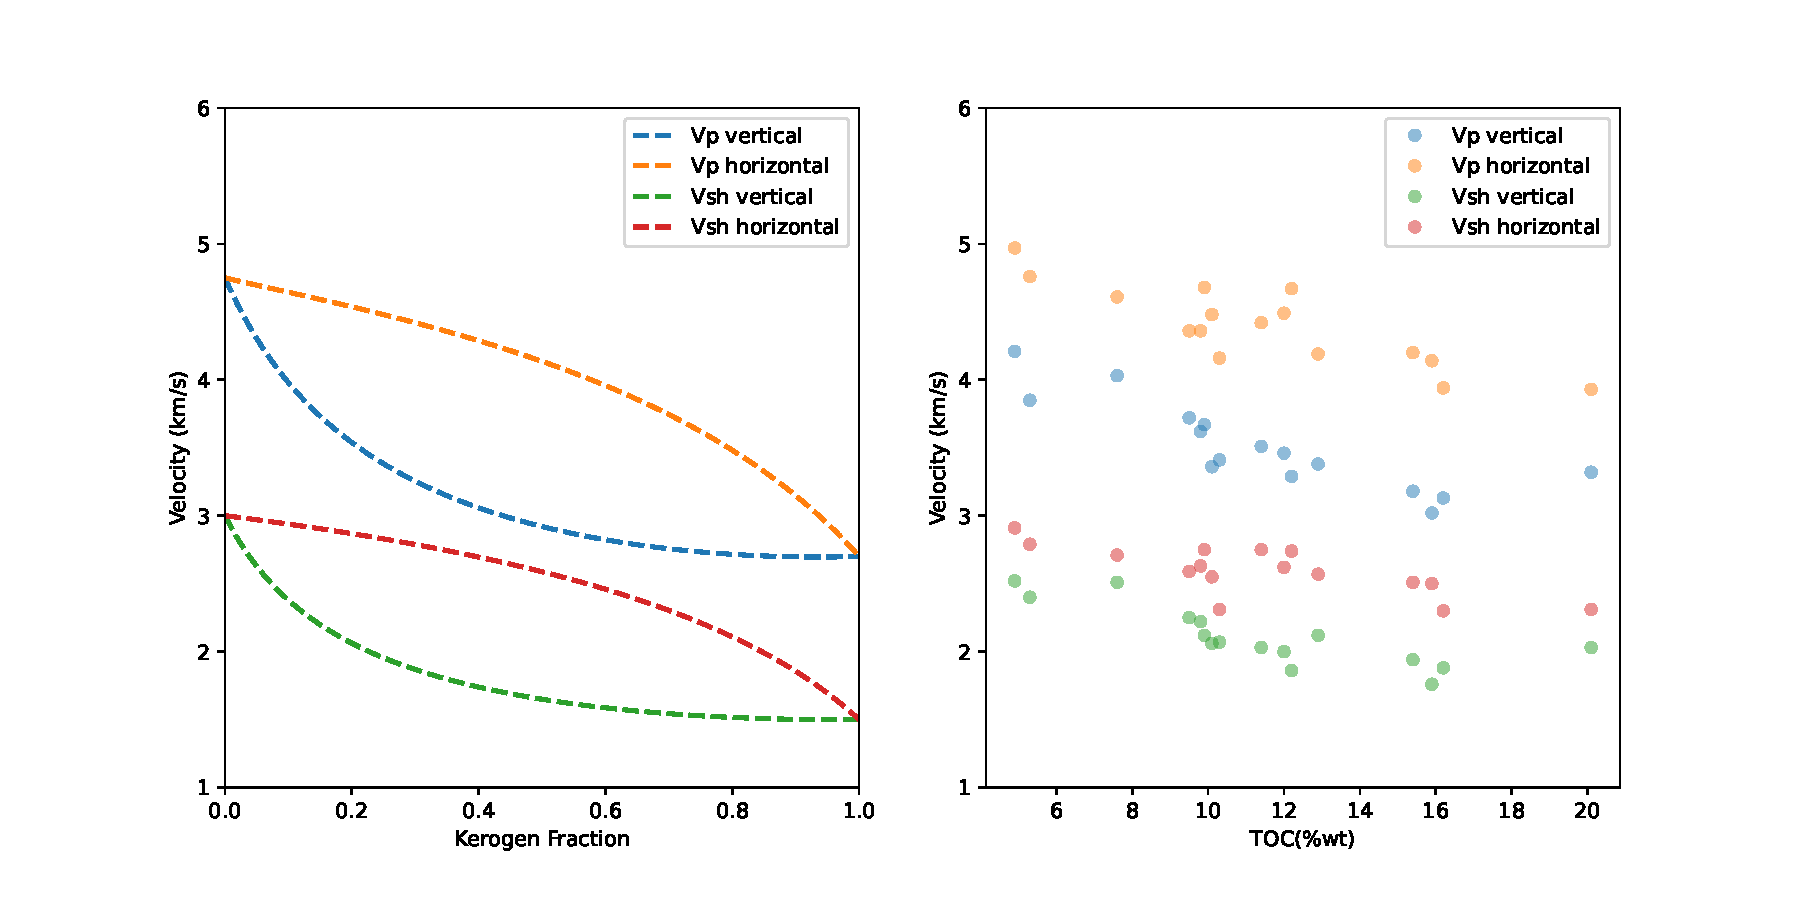
\includegraphics[width=1\textwidth]{figures/homework-2/p3-c.pdf}
        \caption{Predicted and Bakken shale data}
        \label{fig:p3-c}
    \end{figure}
\end{solution}


\begin{problem}{(d)}
    Using the same data and predictions, plot the P and Sh wave anisotropy in terms of the ratio between horizontal (fast) and vertical (slow) velocities. For what kerogen fraction do you expect the maximum levels of anisotropy? Which seismic phase “sees” the greater anisotropy and why might that be the case?
\end{problem}
\begin{solution}
    When the kerogen fraction is 0.5, the anisotropy reaches the maximum.
    The S wave shows more anisotropy than P wave.
    Because the vibration directions of S wave is large different with P wave.
    Two split waves of S wave, one is perpendicular to the cracks, and another is parallel.
    \begin{figure}[H]
        \centering
        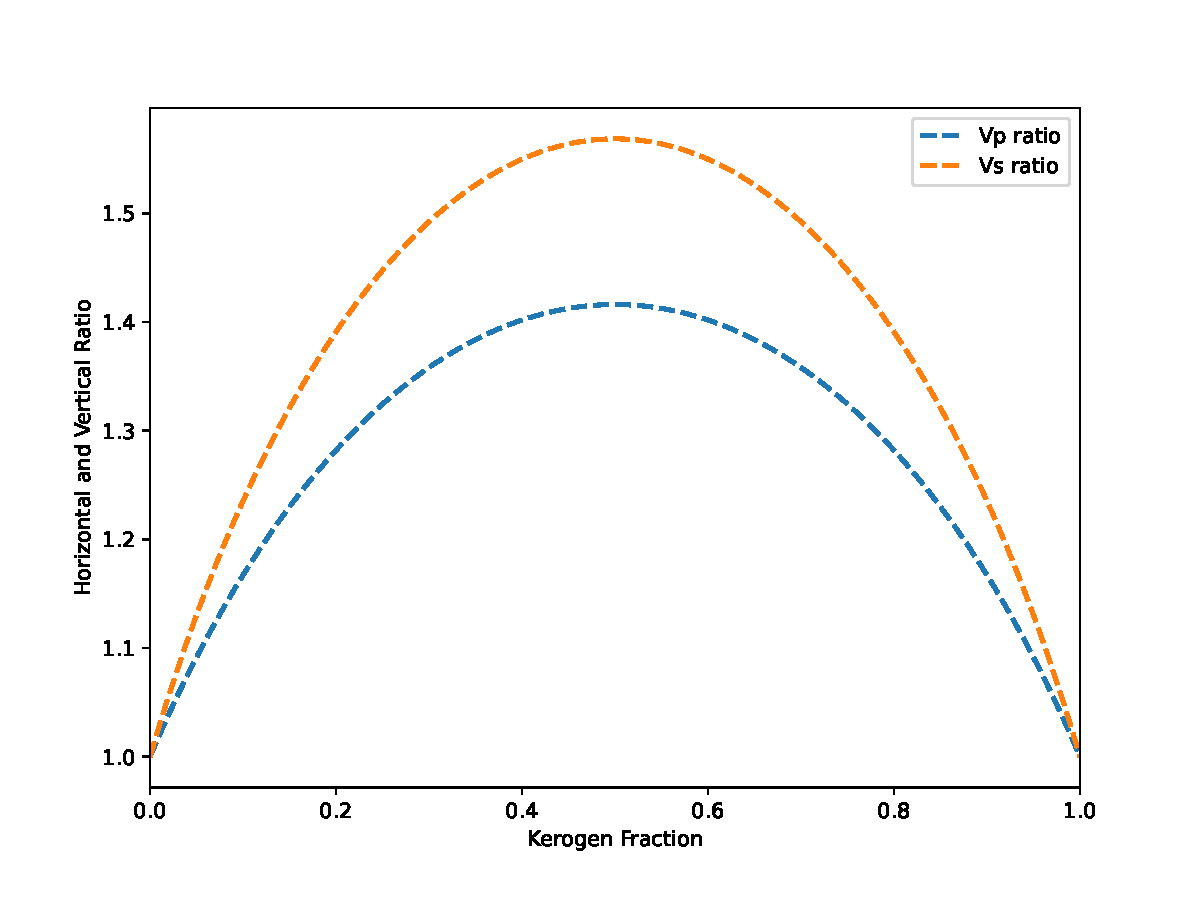
\includegraphics[width=0.8\textwidth]{figures/homework-2/p3-d.pdf}
        \caption{Anisotropy}
        \label{fig:p3-d}
    \end{figure}
\end{solution}

%%%%%%%%%%%%%%%%%%%%%%%%%%%%%%%%%%%%%%%%%%%%%%%%%%%
%                   Scripts
%%%%%%%%%%%%%%%%%%%%%%%%%%%%%%%%%%%%%%%%%%%%%%%%%%%

\section{Scripts}
Noted: I transform jupyter-notebook to python scripts and show it here. 
If you want to run the scripts, I recommended to use original jupyter-notebook scripts instead of transformed python scripts. 

\subsection{Problem-1}

% \begin{pythoncode}
%     import numpy as np
%     """
%         Annotation here.
%     """
%     # Annotation here.
%     def main():
%         for i in range(0,10,1):
%             if i == 1:
%                 print("Hello world")
    
%     # Annotation here.
%     if __name__ == "__main__":
%         main()
% \end{pythoncode}

\pythonfile{figures/homework-2/Problem-1.py}
\subsection{Problem-2}
\pythonfile{figures/homework-2/Problem-2.py}
\subsection{Problem-3}
\pythonfile{figures/homework-2/Problem-3.py}
\clearpage